\newpage
\small
\pagestyle{fancy}
\lhead{\thepage}\chead{ {\bfКВАНТ} $\cdot$ 2010 / \textnumero2}
\begin{multicols}{2}
\noindent– первый катер увеличил скорость до 11 узлов. Второй катер в некоторой точке $B$ уменьшил скорость до 9 узлов, причем на финише выяснилось, что до точки $В$ он плыл ровно половину всего времени. Какая из точек ближе к Дивноморску: $А$ или $B$? Чему равно расстояние $\Delta L$ от точи $А$ до точки $В$? Известно, что расстояние от места старта до финиша $L = 3,6$ мили. Примечание. Один узел – это скорость, при которой судно проходит 1 милю за 1 час.\\
\strut\hfill {\it Фольклор}\\

\quad{\bfЗадача 4. Под микроcкопом.} На рисунке 4 приведено изображение кончика иглы, наблюдаемое в микроскоп. Рас-
\begin{figure}[H]
	\center{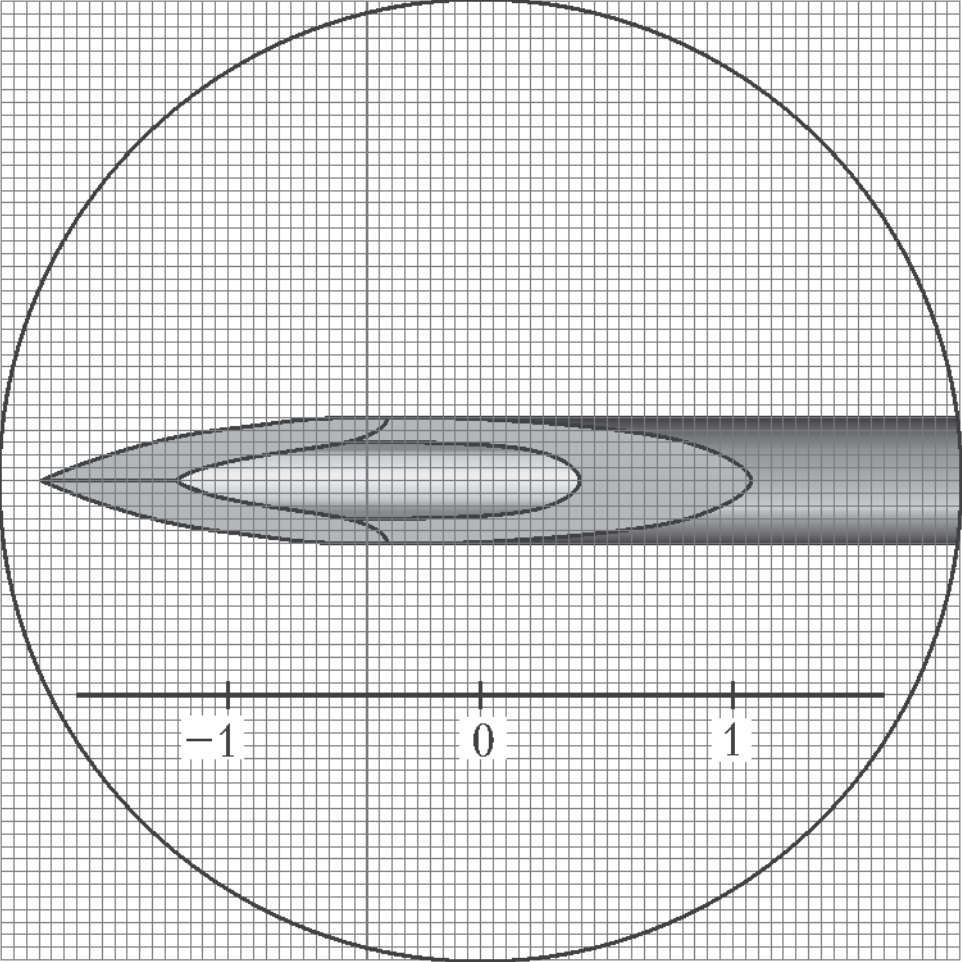
\includegraphics[width=0.35\textwidth]{igla.png}}
\end{figure}
\noindentстояние между делениями 0 и 1 соответствует одному миллиметру. Чему равен внешний диаметр иглы $d$? Найдите также толщину стенок иглы $h$.\\
\strut\hfill {\it И.Ерофеев}
\begin{center}
{\it8 класс}
\end{center}

\quad{\bfЗадача 1. Встреча.} Мальчик стоит на эскалаторе, поднимающемся вверх со скоростью $v$. Ровно на половине пути он поравнялся со своей учительницей, стоящей на соседнем эскалаторе, движущемся вниз с той же скоростью. Как мальчику быстрее добраться до учительницы, если он может двигаться относительно эскалатора с постоянной скоростью $u > 2v$: сначала побежать вверх, сменить эскалатор и побежать вниз или побежать сначала вниз, сменить эскалатор и побежать навстречу вверх?\\
\strut\hfill {\it В. Слободянин}\\

\quad{\bfЗадача 2. Последовательный контакт.} В трех одинаковых теплоизолированных сосудах находятся одинаковые количества масла при комнатной температуре. Нагретый металлический цилиндр опустили в первый сосуд. После того, как между цилиндром и маслом установилось тепловое равновесие, цилиндр перенесли во второй сосуд. После того, как и там установилось равновесие, цилиндр перенесли в  третий сосуд. На сколько градусов повысилась температура масла в третьем сосуде, если во втором она возросла на 5 °C, а в первом – на 20 °C ?\\
\strut\hfill {\it Фольклор}\\

\quad{\bfЗадача 3. Груз на линейке.} Если груз массой $m = 10$ г поставить на расстоянии $х$ от края линейки, то она примет горизонтальное положение равновесия при размещении под ней упора на расстоянии у от того же края линейки (рис.5). Зависимость $y(x)$ при различных размещениях груза пред-\\
\begin{figure}[H]
	\center{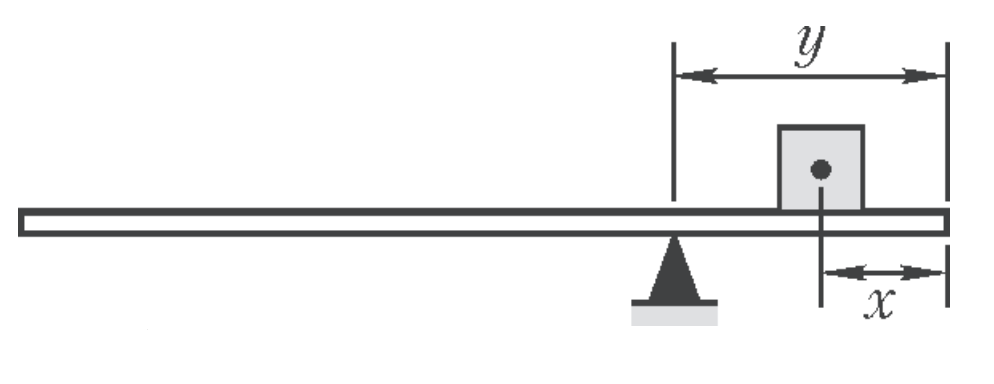
\includegraphics[width=0.3\textwidth]{ruler.png}}
\end{figure}
\noindentставлена в таблице:
\begin{center}
\begin{tabular} {|c|c|c|c|c|c|c|c|}
 \hline
 $x, $мм & 10 & 30 & 50 & 70 & 90 & 100 & 120 \\
 \hline
 $y, $мм & 120 & \multicolumn{2}{l|}{sometext} & 146 & 155 & 160 & 160 \\
\hline
\end{tabular}
\end{center}
Построив график зависимости $y(x)$, определите массу линейки и ее длину.\\
\strut\hfill {\it С.Кармазин}\\

\quad{\bfЗадача 4. Вот он какой, силикатный кирпич!} Силикатный кирпич имеет следующие размеры сторон: $a = 5$ см, $b = $ 10 см и $c = $ 20 см. Два таких кирпича поставили буквой $Т$ сначала
\setlength{\intextsep}{-9pt}
\setlength{\columnsep}{-5pt}
\begin{wrapfigure}{r}{0.75\linewidth}
 \begin{center}
  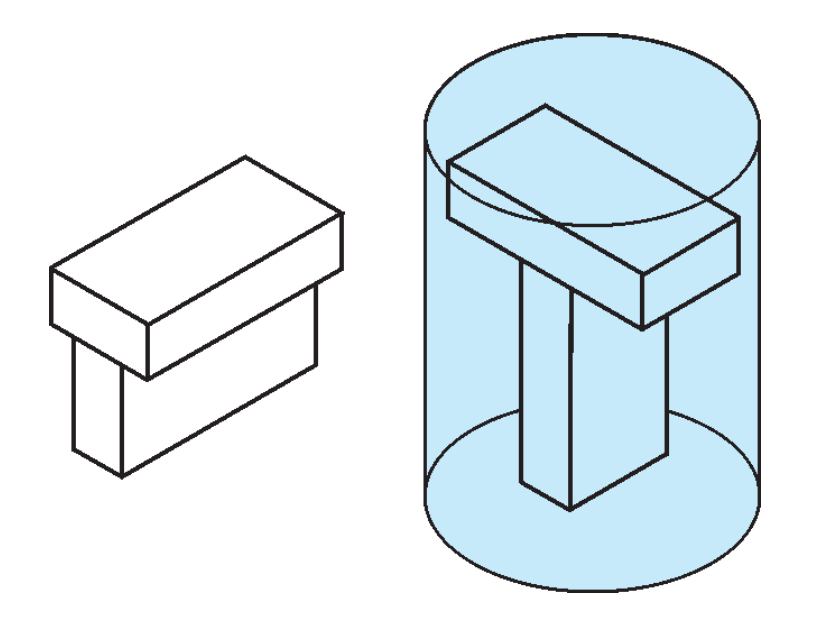
\includegraphics[scale = 0.2]{shapes.png}
 \end{center}
\end{wrapfigure}

\noindentна основание $a\times c$ на стол, а потом на основание $a\times b$ на дно аквариума, заполненного водой (рис.6). В результате оказалось, что давление кирпичей на обе поверхности одно и то же. Найдите массу $m$ такого кирпича. Поскольку кирпич шершавый, вода под него подтекает. Плотность воды $\rho_0 = 1000 \textup{ кг}/\textup{м}^3$.\\
\strut\hfill {\it Фольклор}
\begin{center}
{\it9 класс}
\end{center}

\quad{\bfЗадача 1. Плот и катер.} От пристани «Дубки» экспериментатор Глюк отправился в путешествие по реке на плоту. Ровно через час он причалил к пристани «Грибки», где обнаружил,
что забыл свой рюкзак на пристани «Дубки». К счастью,
Глюк увидел на берегу своего друга – теоретика Бага, у
которого была моторная лодка. На ней друзья поплыли
обратно, забрали рюкзак и вернулись в «Грибки». Сколько
времени моторная лодка плыла против течения, если все
плавание заняло 32 минуты? Мотор лодки в течение всего
плавания работал на полную мощность, а время, которое
потребовалось на подбор рюкзака, пренебрежимо мало.\\
\strut\hfill {\it В.Слободянин}\\

\quad{\bfЗадача 2. Линейная теплоемкость.} Теплоемкость некоторых материалов может зависеть от температуры. Рассмотрим
брусок массой $m1 = 1$ кг, изготовленный из материала,
удельная теплоемкость которого зависит от температуры $t$ по
закону $c = c_1(1+\alpha t)$, где $c_1 = 1,4\cdot 10^3$ Дж/(кг$\cdot$°C), $\alpha = 0,014$ °C$^{-1}$. Такой брусок, нагретый до температуры, опускают в калориметр, в котором находится
некоторая масса $m2$
 воды при температуре $t2$ = ° 20 C . После
установления теплового равновесия температура в калориметре оказалась равной $t0$ = ° 60 C . Пренебрегая теплоемкостью калориметра и тепловыми потерями, определите массу $m2$
 воды в калориметре. Известно, что удельная теплоемкость воды $c_2 = 4,2\cdot10^3$ Дж/(кг$\cdot$°C)\\
 \strut\hfill {\it С.Козел}\\
 
\quad {\bfЗадача 3. Цепь с двумя амперметрами.} В электрической
цепи (рис.7) сила тока, проходящего через резистор сопротивлением $R_3$, равна 1 мА. Сопротивления резисторов
\end{multicols}